% Options for packages loaded elsewhere
\PassOptionsToPackage{unicode}{hyperref}
\PassOptionsToPackage{hyphens}{url}
\PassOptionsToPackage{dvipsnames,svgnames,x11names}{xcolor}
%
\documentclass[
  12pt,
  letterpaper,
  DIV=11,
  numbers=noendperiod]{scrartcl}

\usepackage{amsmath,amssymb}
\usepackage{iftex}
\ifPDFTeX
  \usepackage[T1]{fontenc}
  \usepackage[utf8]{inputenc}
  \usepackage{textcomp} % provide euro and other symbols
\else % if luatex or xetex
  \usepackage{unicode-math}
  \defaultfontfeatures{Scale=MatchLowercase}
  \defaultfontfeatures[\rmfamily]{Ligatures=TeX,Scale=1}
\fi
\usepackage{lmodern}
\ifPDFTeX\else  
    % xetex/luatex font selection
\fi
% Use upquote if available, for straight quotes in verbatim environments
\IfFileExists{upquote.sty}{\usepackage{upquote}}{}
\IfFileExists{microtype.sty}{% use microtype if available
  \usepackage[]{microtype}
  \UseMicrotypeSet[protrusion]{basicmath} % disable protrusion for tt fonts
}{}
\makeatletter
\@ifundefined{KOMAClassName}{% if non-KOMA class
  \IfFileExists{parskip.sty}{%
    \usepackage{parskip}
  }{% else
    \setlength{\parindent}{0pt}
    \setlength{\parskip}{6pt plus 2pt minus 1pt}}
}{% if KOMA class
  \KOMAoptions{parskip=half}}
\makeatother
\usepackage{xcolor}
\setlength{\emergencystretch}{3em} % prevent overfull lines
\setcounter{secnumdepth}{4}
% Make \paragraph and \subparagraph free-standing
\makeatletter
\ifx\paragraph\undefined\else
  \let\oldparagraph\paragraph
  \renewcommand{\paragraph}{
    \@ifstar
      \xxxParagraphStar
      \xxxParagraphNoStar
  }
  \newcommand{\xxxParagraphStar}[1]{\oldparagraph*{#1}\mbox{}}
  \newcommand{\xxxParagraphNoStar}[1]{\oldparagraph{#1}\mbox{}}
\fi
\ifx\subparagraph\undefined\else
  \let\oldsubparagraph\subparagraph
  \renewcommand{\subparagraph}{
    \@ifstar
      \xxxSubParagraphStar
      \xxxSubParagraphNoStar
  }
  \newcommand{\xxxSubParagraphStar}[1]{\oldsubparagraph*{#1}\mbox{}}
  \newcommand{\xxxSubParagraphNoStar}[1]{\oldsubparagraph{#1}\mbox{}}
\fi
\makeatother

\usepackage{color}
\usepackage{fancyvrb}
\newcommand{\VerbBar}{|}
\newcommand{\VERB}{\Verb[commandchars=\\\{\}]}
\DefineVerbatimEnvironment{Highlighting}{Verbatim}{commandchars=\\\{\}}
% Add ',fontsize=\small' for more characters per line
\usepackage{framed}
\definecolor{shadecolor}{RGB}{241,243,245}
\newenvironment{Shaded}{\begin{snugshade}}{\end{snugshade}}
\newcommand{\AlertTok}[1]{\textcolor[rgb]{0.68,0.00,0.00}{#1}}
\newcommand{\AnnotationTok}[1]{\textcolor[rgb]{0.37,0.37,0.37}{#1}}
\newcommand{\AttributeTok}[1]{\textcolor[rgb]{0.40,0.45,0.13}{#1}}
\newcommand{\BaseNTok}[1]{\textcolor[rgb]{0.68,0.00,0.00}{#1}}
\newcommand{\BuiltInTok}[1]{\textcolor[rgb]{0.00,0.23,0.31}{#1}}
\newcommand{\CharTok}[1]{\textcolor[rgb]{0.13,0.47,0.30}{#1}}
\newcommand{\CommentTok}[1]{\textcolor[rgb]{0.37,0.37,0.37}{#1}}
\newcommand{\CommentVarTok}[1]{\textcolor[rgb]{0.37,0.37,0.37}{\textit{#1}}}
\newcommand{\ConstantTok}[1]{\textcolor[rgb]{0.56,0.35,0.01}{#1}}
\newcommand{\ControlFlowTok}[1]{\textcolor[rgb]{0.00,0.23,0.31}{\textbf{#1}}}
\newcommand{\DataTypeTok}[1]{\textcolor[rgb]{0.68,0.00,0.00}{#1}}
\newcommand{\DecValTok}[1]{\textcolor[rgb]{0.68,0.00,0.00}{#1}}
\newcommand{\DocumentationTok}[1]{\textcolor[rgb]{0.37,0.37,0.37}{\textit{#1}}}
\newcommand{\ErrorTok}[1]{\textcolor[rgb]{0.68,0.00,0.00}{#1}}
\newcommand{\ExtensionTok}[1]{\textcolor[rgb]{0.00,0.23,0.31}{#1}}
\newcommand{\FloatTok}[1]{\textcolor[rgb]{0.68,0.00,0.00}{#1}}
\newcommand{\FunctionTok}[1]{\textcolor[rgb]{0.28,0.35,0.67}{#1}}
\newcommand{\ImportTok}[1]{\textcolor[rgb]{0.00,0.46,0.62}{#1}}
\newcommand{\InformationTok}[1]{\textcolor[rgb]{0.37,0.37,0.37}{#1}}
\newcommand{\KeywordTok}[1]{\textcolor[rgb]{0.00,0.23,0.31}{\textbf{#1}}}
\newcommand{\NormalTok}[1]{\textcolor[rgb]{0.00,0.23,0.31}{#1}}
\newcommand{\OperatorTok}[1]{\textcolor[rgb]{0.37,0.37,0.37}{#1}}
\newcommand{\OtherTok}[1]{\textcolor[rgb]{0.00,0.23,0.31}{#1}}
\newcommand{\PreprocessorTok}[1]{\textcolor[rgb]{0.68,0.00,0.00}{#1}}
\newcommand{\RegionMarkerTok}[1]{\textcolor[rgb]{0.00,0.23,0.31}{#1}}
\newcommand{\SpecialCharTok}[1]{\textcolor[rgb]{0.37,0.37,0.37}{#1}}
\newcommand{\SpecialStringTok}[1]{\textcolor[rgb]{0.13,0.47,0.30}{#1}}
\newcommand{\StringTok}[1]{\textcolor[rgb]{0.13,0.47,0.30}{#1}}
\newcommand{\VariableTok}[1]{\textcolor[rgb]{0.07,0.07,0.07}{#1}}
\newcommand{\VerbatimStringTok}[1]{\textcolor[rgb]{0.13,0.47,0.30}{#1}}
\newcommand{\WarningTok}[1]{\textcolor[rgb]{0.37,0.37,0.37}{\textit{#1}}}

\providecommand{\tightlist}{%
  \setlength{\itemsep}{0pt}\setlength{\parskip}{0pt}}\usepackage{longtable,booktabs,array}
\usepackage{calc} % for calculating minipage widths
% Correct order of tables after \paragraph or \subparagraph
\usepackage{etoolbox}
\makeatletter
\patchcmd\longtable{\par}{\if@noskipsec\mbox{}\fi\par}{}{}
\makeatother
% Allow footnotes in longtable head/foot
\IfFileExists{footnotehyper.sty}{\usepackage{footnotehyper}}{\usepackage{footnote}}
\makesavenoteenv{longtable}
\usepackage{graphicx}
\makeatletter
\newsavebox\pandoc@box
\newcommand*\pandocbounded[1]{% scales image to fit in text height/width
  \sbox\pandoc@box{#1}%
  \Gscale@div\@tempa{\textheight}{\dimexpr\ht\pandoc@box+\dp\pandoc@box\relax}%
  \Gscale@div\@tempb{\linewidth}{\wd\pandoc@box}%
  \ifdim\@tempb\p@<\@tempa\p@\let\@tempa\@tempb\fi% select the smaller of both
  \ifdim\@tempa\p@<\p@\scalebox{\@tempa}{\usebox\pandoc@box}%
  \else\usebox{\pandoc@box}%
  \fi%
}
% Set default figure placement to htbp
\def\fps@figure{htbp}
\makeatother

\usepackage{booktabs}
\usepackage{longtable}
\usepackage{array}
\usepackage{multirow}
\usepackage{wrapfig}
\usepackage{float}
\usepackage{colortbl}
\usepackage{pdflscape}
\usepackage{tabu}
\usepackage{threeparttable}
\usepackage{threeparttablex}
\usepackage[normalem]{ulem}
\usepackage{makecell}
\usepackage{xcolor}
\KOMAoption{captions}{tableheading}
\makeatletter
\@ifpackageloaded{caption}{}{\usepackage{caption}}
\AtBeginDocument{%
\ifdefined\contentsname
  \renewcommand*\contentsname{Table of contents}
\else
  \newcommand\contentsname{Table of contents}
\fi
\ifdefined\listfigurename
  \renewcommand*\listfigurename{List of Figures}
\else
  \newcommand\listfigurename{List of Figures}
\fi
\ifdefined\listtablename
  \renewcommand*\listtablename{List of Tables}
\else
  \newcommand\listtablename{List of Tables}
\fi
\ifdefined\figurename
  \renewcommand*\figurename{Figure}
\else
  \newcommand\figurename{Figure}
\fi
\ifdefined\tablename
  \renewcommand*\tablename{Table}
\else
  \newcommand\tablename{Table}
\fi
}
\@ifpackageloaded{float}{}{\usepackage{float}}
\floatstyle{ruled}
\@ifundefined{c@chapter}{\newfloat{codelisting}{h}{lop}}{\newfloat{codelisting}{h}{lop}[chapter]}
\floatname{codelisting}{Listing}
\newcommand*\listoflistings{\listof{codelisting}{List of Listings}}
\makeatother
\makeatletter
\makeatother
\makeatletter
\@ifpackageloaded{caption}{}{\usepackage{caption}}
\@ifpackageloaded{subcaption}{}{\usepackage{subcaption}}
\makeatother

\usepackage{bookmark}

\IfFileExists{xurl.sty}{\usepackage{xurl}}{} % add URL line breaks if available
\urlstyle{same} % disable monospaced font for URLs
\hypersetup{
  pdftitle={Real Dataset Analysis},
  colorlinks=true,
  linkcolor={blue},
  filecolor={Maroon},
  citecolor={Blue},
  urlcolor={Blue},
  pdfcreator={LaTeX via pandoc}}


\title{Real Dataset Analysis}
\author{}
\date{}

\begin{document}
\maketitle


\begin{Shaded}
\begin{Highlighting}[]
\CommentTok{\# Load preprocessed dataset}
\NormalTok{bladder\_comp\_adj }\OtherTok{\textless{}{-}} \FunctionTok{readRDS}\NormalTok{(}\FunctionTok{here}\NormalTok{(}\StringTok{"paper"}\NormalTok{, }\StringTok{"data"}\NormalTok{, }\StringTok{"bladder\_comp\_adj.rds"}\NormalTok{))}

\CommentTok{\# Create a stratified 75/25 split}
\FunctionTok{set.seed}\NormalTok{(}\DecValTok{1234}\NormalTok{)}
\NormalTok{split }\OtherTok{\textless{}{-}} \FunctionTok{initial\_split}\NormalTok{(bladder\_comp\_adj, }\AttributeTok{prop =} \FloatTok{0.75}\NormalTok{, }\AttributeTok{strata =}\NormalTok{ event)}

\CommentTok{\# Create training and testing data frames}
\NormalTok{train }\OtherTok{\textless{}{-}} \FunctionTok{training}\NormalTok{(split)}
\NormalTok{test  }\OtherTok{\textless{}{-}} \FunctionTok{testing}\NormalTok{(split)}

\CommentTok{\# Verify the proportions}
\FunctionTok{table}\NormalTok{(train}\SpecialCharTok{$}\NormalTok{event) }\SpecialCharTok{/} \FunctionTok{nrow}\NormalTok{(train)}
\end{Highlighting}
\end{Shaded}

\begin{verbatim}
#> 
#>          0          1          2 
#> 0.75111111 0.07111111 0.17777778
\end{verbatim}

\begin{Shaded}
\begin{Highlighting}[]
\FunctionTok{table}\NormalTok{(test}\SpecialCharTok{$}\NormalTok{event) }\SpecialCharTok{/} \FunctionTok{nrow}\NormalTok{(test)}
\end{Highlighting}
\end{Shaded}

\begin{verbatim}
#> 
#>          0          1          2 
#> 0.76315789 0.05263158 0.18421053
\end{verbatim}

\section{Analysis without Clinical
Vars}\label{analysis-without-clinical-vars}

TESTING

\subsection{cbSCRIP}\label{cbscrip}

\begin{Shaded}
\begin{Highlighting}[]
\CommentTok{\# Set fitting parameters}
\ControlFlowTok{if}\NormalTok{(save)\{}
    
    \FunctionTok{set.seed}\NormalTok{(}\DecValTok{123}\NormalTok{)}
    
\NormalTok{    cv\_nc }\OtherTok{\textless{}{-}} \FunctionTok{cv\_cbSCRIP}\NormalTok{(}
        \FunctionTok{Surv}\NormalTok{(time, event) }\SpecialCharTok{\textasciitilde{}}\NormalTok{ .,}
\NormalTok{        train[,}\SpecialCharTok{{-}}\NormalTok{(}\DecValTok{3}\SpecialCharTok{:}\DecValTok{7}\NormalTok{), , }\AttributeTok{drop =} \ConstantTok{FALSE}\NormalTok{],}
        \AttributeTok{alpha =} \FloatTok{0.7}\NormalTok{,}
        \AttributeTok{nfold =} \DecValTok{5}\NormalTok{,}
        \AttributeTok{nlambda =} \DecValTok{50}\NormalTok{,}
        \AttributeTok{ratio =} \DecValTok{50}\NormalTok{)}
    
    \FunctionTok{plot}\NormalTok{(cv\_nc)}
    
    \FunctionTok{saveRDS}\NormalTok{(cv\_nc, }\FunctionTok{here}\NormalTok{(}\StringTok{"paper"}\NormalTok{,}
                 \StringTok{"results"}\NormalTok{,}
                 \FunctionTok{glue}\NormalTok{(}\StringTok{"cv\_nc.rds"}\NormalTok{)))}
\NormalTok{\}}

\NormalTok{cv\_nc }\OtherTok{\textless{}{-}} \FunctionTok{readRDS}\NormalTok{(}\FunctionTok{here}\NormalTok{(}\StringTok{"paper"}\NormalTok{, }\StringTok{"results"}\NormalTok{, }\FunctionTok{glue}\NormalTok{(}\StringTok{"cv\_nc.rds"}\NormalTok{)))}

\CommentTok{\# Print c{-}plot}
\FunctionTok{plot}\NormalTok{(cv\_nc)}
\end{Highlighting}
\end{Shaded}

\begin{center}
\pandocbounded{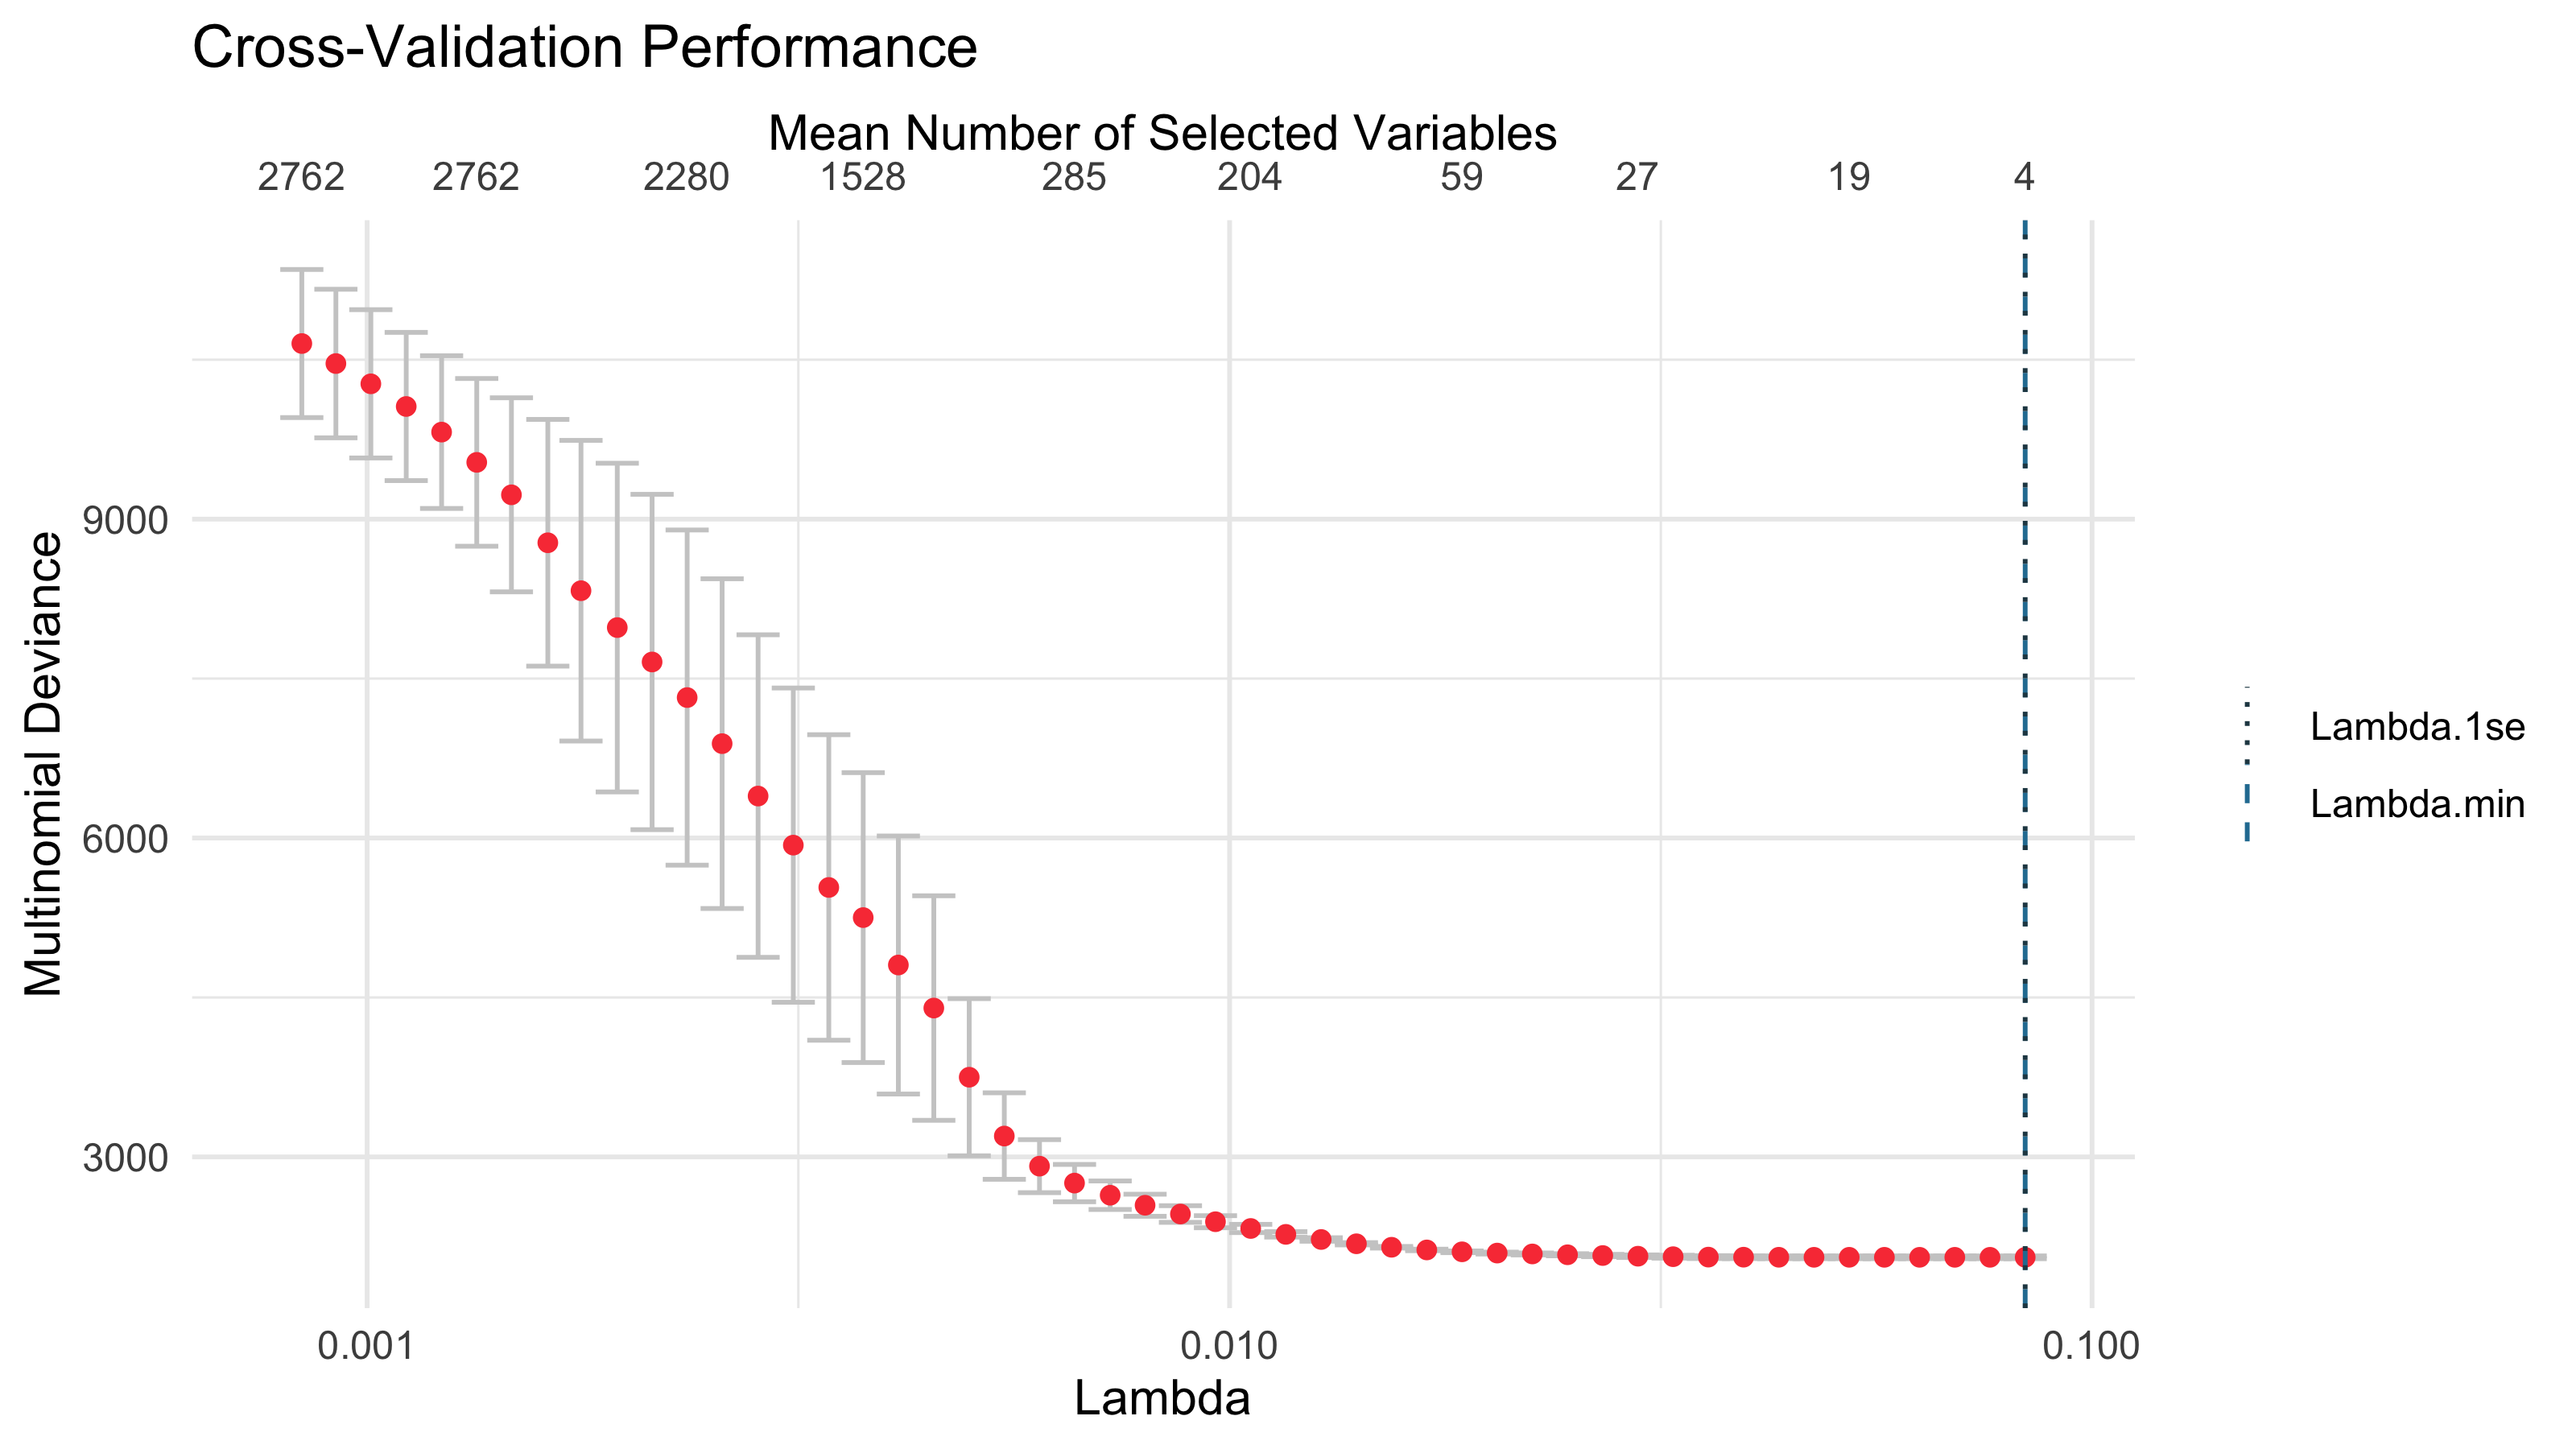
\includegraphics[keepaspectratio]{selection-1SE_files/figure-pdf/unnamed-chunk-2-1.png}}
\end{center}

\begin{Shaded}
\begin{Highlighting}[]
\CommentTok{\# Print selected vars}
\DocumentationTok{\#\# filter rows}
\NormalTok{filt\_rows }\OtherTok{\textless{}{-}} \FunctionTok{which}\NormalTok{(}\SpecialCharTok{!}\FunctionTok{same}\NormalTok{(cv\_nc}\SpecialCharTok{$}\NormalTok{fit.min}\SpecialCharTok{$}\NormalTok{coefficients[,}\DecValTok{1}\NormalTok{], }\DecValTok{0}\NormalTok{) }\SpecialCharTok{|} 
          \SpecialCharTok{!}\FunctionTok{same}\NormalTok{(cv\_nc}\SpecialCharTok{$}\NormalTok{fit.min}\SpecialCharTok{$}\NormalTok{coefficients[,}\DecValTok{2}\NormalTok{], }\DecValTok{0}\NormalTok{)) }

\NormalTok{cv\_nc}\SpecialCharTok{$}\NormalTok{fit.min}\SpecialCharTok{$}\NormalTok{coefficients[filt\_rows,]}
\end{Highlighting}
\end{Shaded}

\begin{verbatim}
#>                   [,1]       [,2]
#> log(time)   -0.4213303 -0.5532271
#> (Intercept) -4.9795840 -4.0324360
\end{verbatim}

\begin{Shaded}
\begin{Highlighting}[]
\CommentTok{\# Fit model with Lambda(min + 1SE)}
\NormalTok{lambda\_min\_nc }\OtherTok{\textless{}{-}}\NormalTok{ cv\_nc}\SpecialCharTok{$}\NormalTok{lambda.min}
\NormalTok{lambda\_min\_nc\_idx }\OtherTok{\textless{}{-}} \FunctionTok{which}\NormalTok{(lambda\_min\_nc }\SpecialCharTok{==}\NormalTok{ cv\_nc}\SpecialCharTok{$}\NormalTok{lambdagrid)}
\NormalTok{dev\_lambda\_nc }\OtherTok{\textless{}{-}}\NormalTok{ cv\_nc}\SpecialCharTok{$}\NormalTok{deviance\_mean[lambda\_min\_nc\_idx]}
\NormalTok{se\_lambda\_nc }\OtherTok{\textless{}{-}}\NormalTok{ cv\_nc}\SpecialCharTok{$}\NormalTok{deviance\_se[lambda\_min\_nc\_idx]}
\NormalTok{lambda\_min\_minus\_se\_idx }\OtherTok{\textless{}{-}} \FunctionTok{which.min}\NormalTok{(}\FunctionTok{abs}\NormalTok{(cv\_nc}\SpecialCharTok{$}\NormalTok{deviance\_mean }\SpecialCharTok{{-}}\NormalTok{ (dev\_lambda\_nc }\SpecialCharTok{+}\NormalTok{ se\_lambda\_nc)))}
\NormalTok{lambda\_min\_minus\_se }\OtherTok{\textless{}{-}}\NormalTok{ cv\_nc}\SpecialCharTok{$}\NormalTok{lambdagrid[lambda\_min\_minus\_se\_idx]}

\CommentTok{\# Fit model with Lambda(min + 1SE)}
\NormalTok{p1se\_nc }\OtherTok{\textless{}{-}} \FunctionTok{cbSCRIP}\NormalTok{(}
        \AttributeTok{cb\_data =}\NormalTok{ cv\_nc}\SpecialCharTok{$}\NormalTok{cb\_data, }\CommentTok{\# using case{-}base sample generated by cv function}
        \AttributeTok{alpha =} \FloatTok{0.7}\NormalTok{,}
        \AttributeTok{lambda =}\NormalTok{ lambda\_min\_minus\_se,}
        \AttributeTok{ratio =} \DecValTok{50}\NormalTok{)}

\CommentTok{\# Print selected vars}
\NormalTok{filt\_rows\_p1se }\OtherTok{\textless{}{-}} \FunctionTok{which}\NormalTok{(}\SpecialCharTok{!}\FunctionTok{same}\NormalTok{(p1se\_nc}\SpecialCharTok{$}\NormalTok{coefficients[[}\DecValTok{1}\NormalTok{]][,}\DecValTok{1}\NormalTok{], }\DecValTok{0}\NormalTok{) }\SpecialCharTok{|} 
          \SpecialCharTok{!}\FunctionTok{same}\NormalTok{(p1se\_nc}\SpecialCharTok{$}\NormalTok{coefficients[[}\DecValTok{1}\NormalTok{]][,}\DecValTok{2}\NormalTok{], }\DecValTok{0}\NormalTok{)) }

\NormalTok{p1se\_nc}\SpecialCharTok{$}\NormalTok{coefficients[[}\DecValTok{1}\NormalTok{]][filt\_rows\_p1se,]}
\end{Highlighting}
\end{Shaded}

\begin{verbatim}
#>                   [,1]        [,2]
#> seq1082      0.0000000  0.00000007
#> seq1225      0.0000000 -0.10569818
#> seq1226      0.0000000 -0.03279161
#> seq240       0.0000000 -0.07337141
#> seq249       0.0000000 -0.06391992
#> seq265       0.0000000  0.00840748
#> seq279       0.0000000 -0.03556827
#> seq302       0.0000000 -0.04444657
#> seq336       0.0000000  0.09603041
#> seq339       0.0000000  0.01441133
#> seq34        0.0000000  0.25704495
#> seq377       0.0000000  0.11540046
#> seq435       0.0000000  0.00475894
#> seq813       0.0000000 -0.14208461
#> seq833       0.0000000  0.14095540
#> seq869       0.0000000 -0.00000004
#> seq972       0.0000000  0.08012004
#> seq973       0.0000000  0.09432033
#> seq982       0.0000000  0.14432298
#> log(time)   -0.5472919 -0.60817172
#> (Intercept) -4.5734631 -3.29665596
\end{verbatim}

\begin{Shaded}
\begin{Highlighting}[]
\CommentTok{\# Repear refitting multiple times}

\ControlFlowTok{if}\NormalTok{(save)\{}
    
    \FunctionTok{set.seed}\NormalTok{(}\DecValTok{123}\NormalTok{)}
    
    \ControlFlowTok{for}\NormalTok{ (i }\ControlFlowTok{in} \DecValTok{1}\SpecialCharTok{:}\DecValTok{50}\NormalTok{) \{}
\NormalTok{    p1se\_nc }\OtherTok{\textless{}{-}} \FunctionTok{cbSCRIP}\NormalTok{(}
        \FunctionTok{Surv}\NormalTok{(time, event) }\SpecialCharTok{\textasciitilde{}}\NormalTok{ .,}
\NormalTok{        train[,}\SpecialCharTok{{-}}\NormalTok{(}\DecValTok{3}\SpecialCharTok{:}\DecValTok{7}\NormalTok{), , }\AttributeTok{drop =} \ConstantTok{FALSE}\NormalTok{],}
        \AttributeTok{alpha =} \FloatTok{0.7}\NormalTok{,}
        \AttributeTok{lambda =}\NormalTok{ lambda\_min\_minus\_se,}
        \AttributeTok{ratio =} \DecValTok{50}\NormalTok{)}
    
    \ControlFlowTok{if}\NormalTok{(i}\SpecialCharTok{==} \DecValTok{1}\NormalTok{) \{}
\NormalTok{        count\_mtx }\OtherTok{\textless{}{-}} \SpecialCharTok{!}\FunctionTok{same}\NormalTok{(p1se\_nc}\SpecialCharTok{$}\NormalTok{coefficients[[}\DecValTok{1}\NormalTok{]],}\DecValTok{0}\NormalTok{)}
\NormalTok{        count\_mtx[] }\OtherTok{\textless{}{-}} \FunctionTok{as.integer}\NormalTok{(}\SpecialCharTok{!}\FunctionTok{same}\NormalTok{(p1se\_nc}\SpecialCharTok{$}\NormalTok{coefficients[[}\DecValTok{1}\NormalTok{]],}\DecValTok{0}\NormalTok{))}
\NormalTok{    \} }\ControlFlowTok{else}\NormalTok{ \{}
\NormalTok{        count\_mtx\_loop }\OtherTok{\textless{}{-}} \SpecialCharTok{!}\FunctionTok{same}\NormalTok{(p1se\_nc}\SpecialCharTok{$}\NormalTok{coefficients[[}\DecValTok{1}\NormalTok{]],}\DecValTok{0}\NormalTok{)}
\NormalTok{        count\_mtx\_loop[] }\OtherTok{\textless{}{-}} \FunctionTok{as.integer}\NormalTok{(}\SpecialCharTok{!}\FunctionTok{same}\NormalTok{(p1se\_nc}\SpecialCharTok{$}\NormalTok{coefficients[[}\DecValTok{1}\NormalTok{]],}\DecValTok{0}\NormalTok{))}
\NormalTok{        count\_mtx[] }\OtherTok{\textless{}{-}}\NormalTok{ count\_mtx }\SpecialCharTok{+}\NormalTok{ count\_mtx\_loop}
\NormalTok{    \}}
    
\NormalTok{    \}}
    
    \FunctionTok{saveRDS}\NormalTok{(count\_mtx, }\FunctionTok{here}\NormalTok{(}\StringTok{"paper"}\NormalTok{,}
                 \StringTok{"results"}\NormalTok{,}
                 \FunctionTok{glue}\NormalTok{(}\StringTok{"count\_mtx.rds"}\NormalTok{)))}
\NormalTok{\}}

\NormalTok{count\_mtx }\OtherTok{\textless{}{-}} \FunctionTok{readRDS}\NormalTok{(}\FunctionTok{here}\NormalTok{(}\StringTok{"paper"}\NormalTok{, }\StringTok{"results"}\NormalTok{, }\FunctionTok{glue}\NormalTok{(}\StringTok{"count\_mtx.rds"}\NormalTok{)))}

\NormalTok{filt\_rows }\OtherTok{\textless{}{-}} \FunctionTok{which}\NormalTok{(}\SpecialCharTok{!}\FunctionTok{same}\NormalTok{(count\_mtx[,}\DecValTok{1}\NormalTok{], }\DecValTok{0}\NormalTok{) }\SpecialCharTok{|} 
          \SpecialCharTok{!}\FunctionTok{same}\NormalTok{(count\_mtx[,}\DecValTok{2}\NormalTok{], }\DecValTok{0}\NormalTok{)) }

\CommentTok{\# Number of variables selected out of 50}
\NormalTok{count\_mtx[filt\_rows,] }
\end{Highlighting}
\end{Shaded}

\begin{verbatim}
#>             [,1] [,2]
#> seq1014        0    3
#> seq1029        0    1
#> seq1031        0    1
#> seq1082        0    8
#> seq1145        0    1
#> seq1177        0   29
#> seq1225        0    9
#> seq1226        0   12
#> seq1227        0    1
#> seq1262        0   12
#> seq1310        0    4
#> seq1364        0    1
#> seq1384_2      0   33
#> seq227         0    1
#> seq240         0   40
#> seq249         0   13
#> seq265         0   50
#> seq279         0   36
#> seq324         0    6
#> seq336         0   18
#> seq339         0   40
#> seq34          0   50
#> seq370         0   24
#> seq377         0   50
#> seq408         0    3
#> seq435         0   14
#> seq438         0    1
#> seq440         0   10
#> seq445         0    2
#> seq49          0    1
#> seq542         0    1
#> seq62          0    1
#> seq681         0    1
#> seq78          0    2
#> seq782         0    2
#> seq793         0    1
#> seq813         0   44
#> seq820         0   11
#> seq833         0   34
#> seq866         0    1
#> seq869         0   10
#> seq919         0    1
#> seq940         0    3
#> seq963         0   13
#> seq972         0   48
#> seq973         0   41
#> seq982         0   31
#> log(time)     50   50
#> (Intercept)   50   50
\end{verbatim}

\subsection{Cox elastic-net}\label{cox-elastic-net}

\begin{Shaded}
\begin{Highlighting}[]
\NormalTok{y }\OtherTok{\textless{}{-}} \FunctionTok{Surv}\NormalTok{(}\AttributeTok{time =}\NormalTok{ train}\SpecialCharTok{$}\NormalTok{time, }
          \AttributeTok{event =} \FunctionTok{as.numeric}\NormalTok{(train}\SpecialCharTok{$}\NormalTok{event }\SpecialCharTok{==} \DecValTok{1}\NormalTok{))}

\NormalTok{x }\OtherTok{\textless{}{-}} \FunctionTok{model.matrix}\NormalTok{(event }\SpecialCharTok{\textasciitilde{}}\NormalTok{ . }\SpecialCharTok{{-}}\NormalTok{time,}
                  \AttributeTok{data =}\NormalTok{ train[,}\SpecialCharTok{{-}}\NormalTok{(}\DecValTok{3}\SpecialCharTok{:}\DecValTok{7}\NormalTok{), , }\AttributeTok{drop =} \ConstantTok{FALSE}\NormalTok{])}

\FunctionTok{set.seed}\NormalTok{(}\DecValTok{1234}\NormalTok{)}
\NormalTok{cox\_enet\_nc }\OtherTok{\textless{}{-}} \FunctionTok{cv.glmnet}\NormalTok{(}\AttributeTok{x =}\NormalTok{ x, }\AttributeTok{y =}\NormalTok{ y, }\AttributeTok{family =} \StringTok{"cox"}\NormalTok{,}
                         \CommentTok{\# family = "binomial",}
                         \AttributeTok{nfolds =} \DecValTok{5}\NormalTok{,}
                         \AttributeTok{alpha =} \FloatTok{0.7}\NormalTok{)}

\FunctionTok{plot}\NormalTok{(cox\_enet\_nc)}
\end{Highlighting}
\end{Shaded}

\begin{center}
\pandocbounded{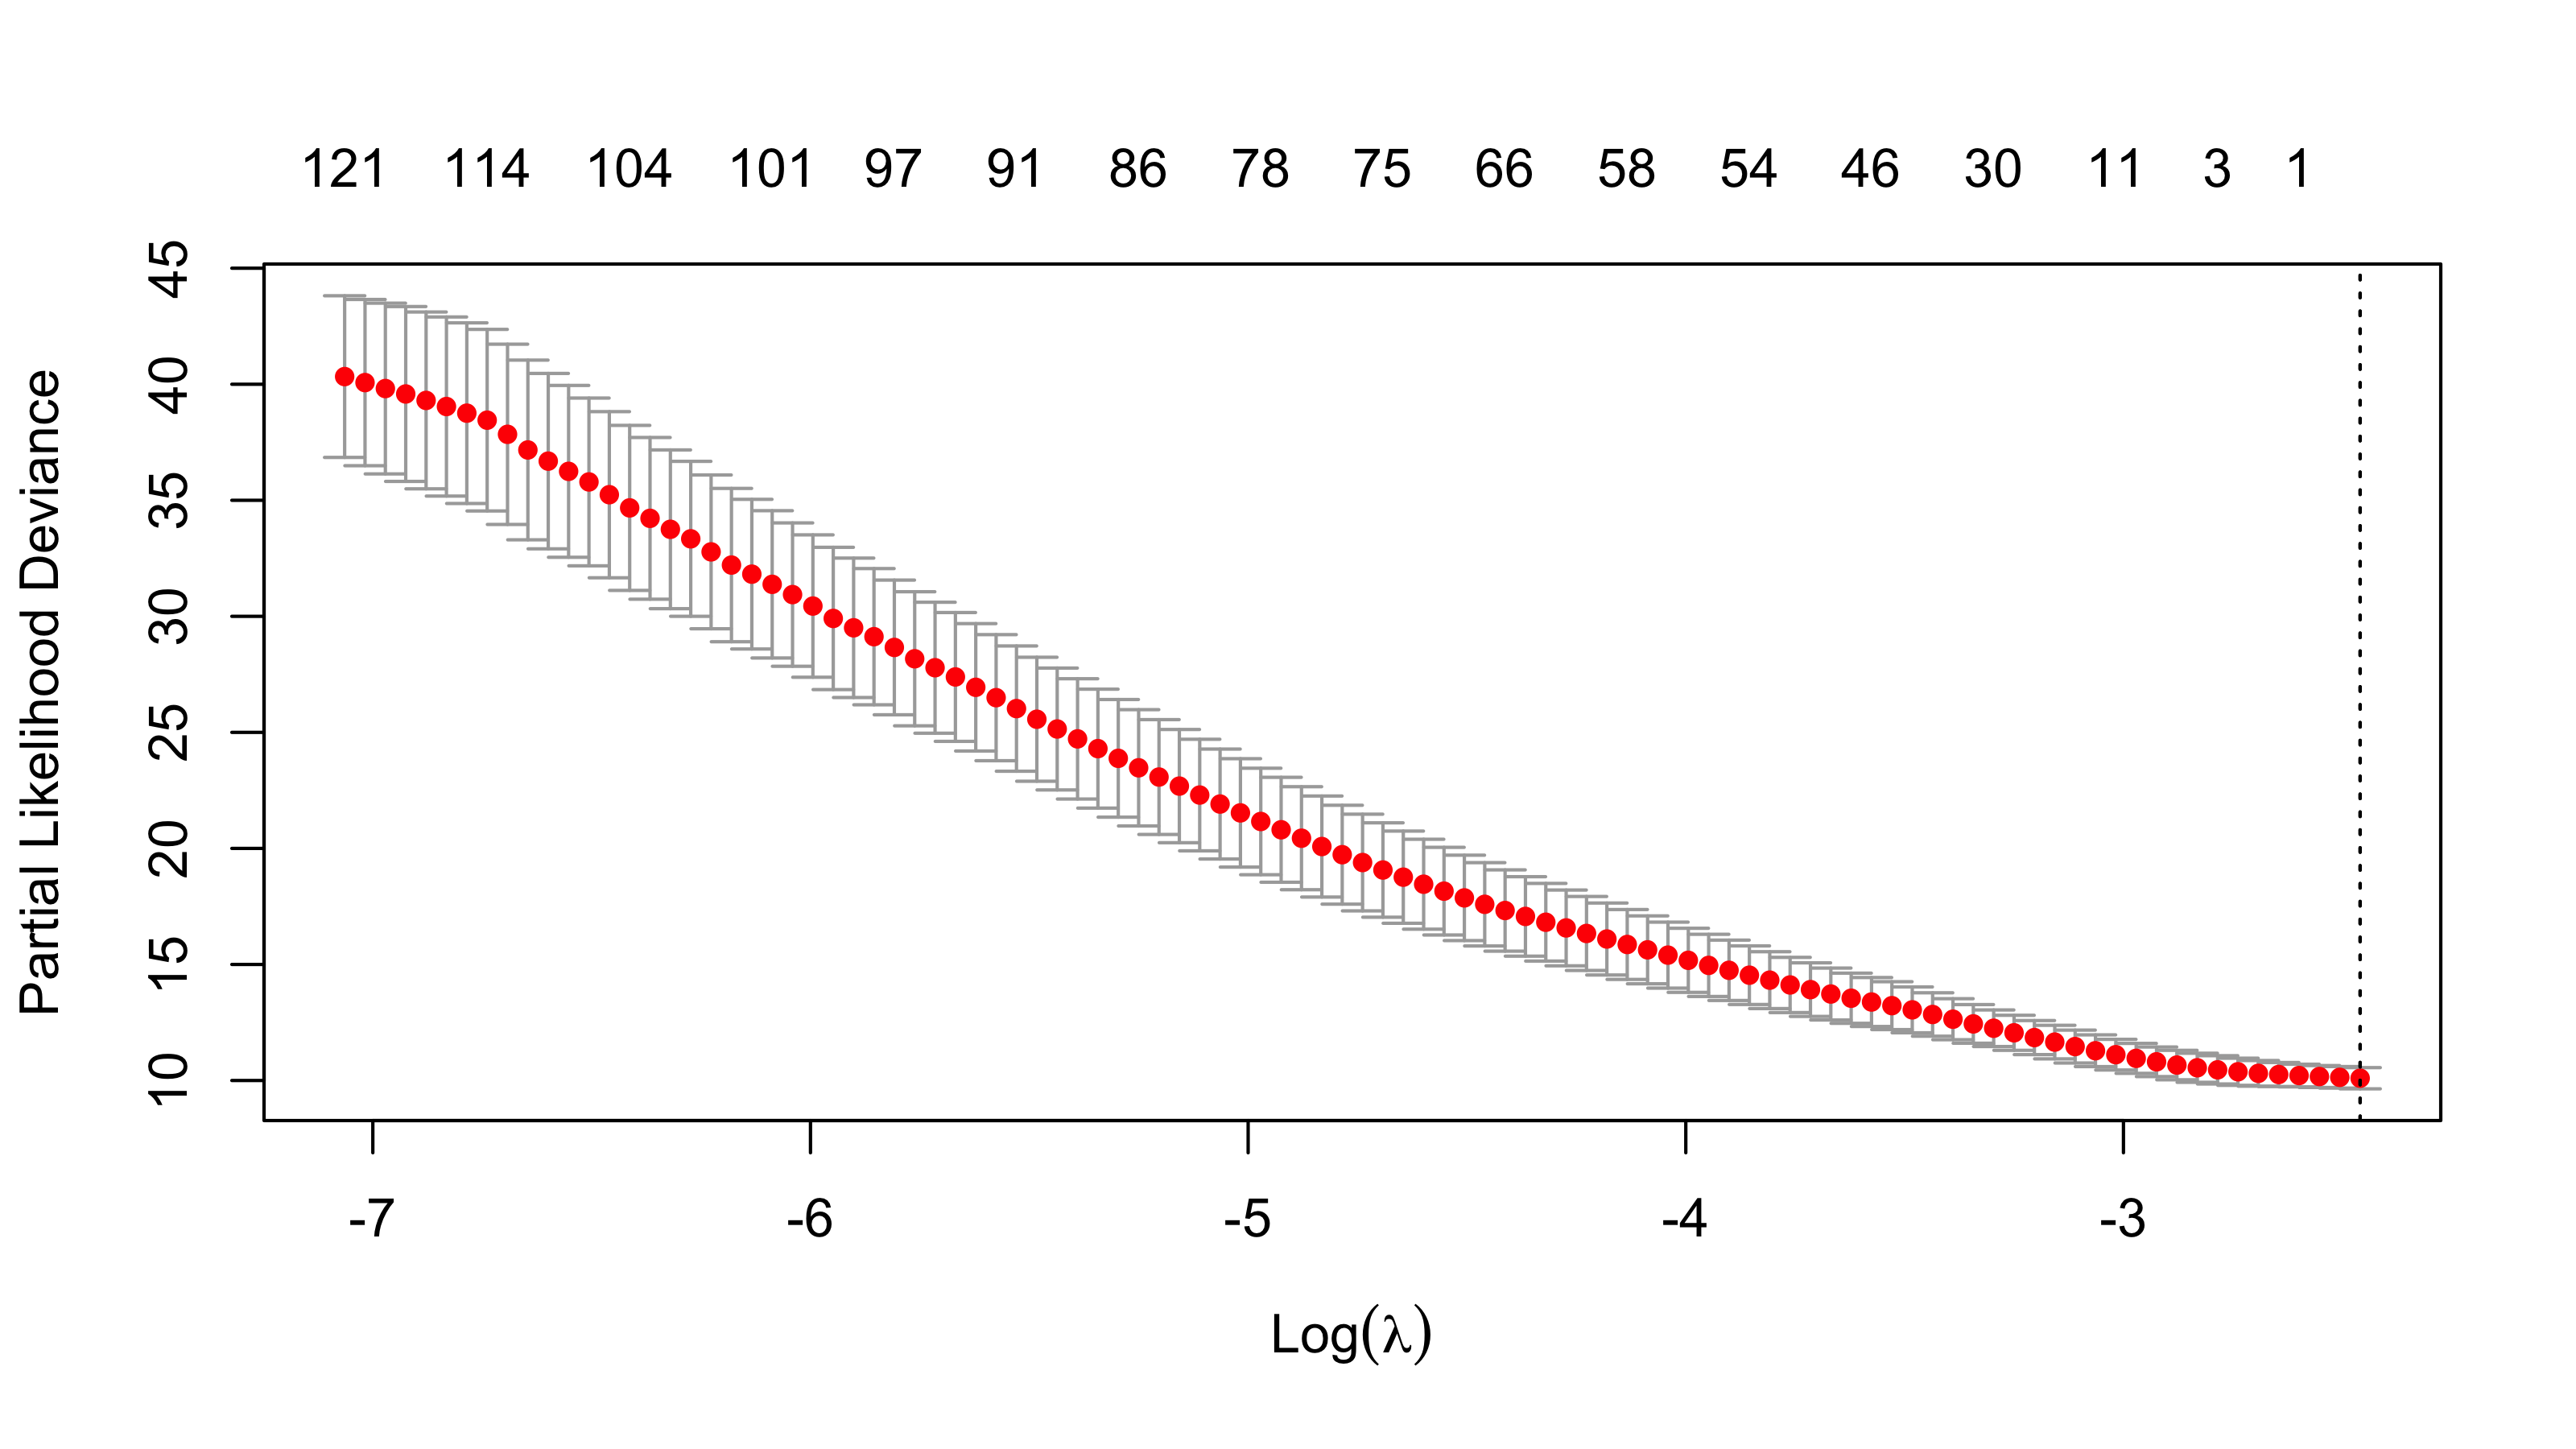
\includegraphics[keepaspectratio]{selection-1SE_files/figure-pdf/unnamed-chunk-3-1.png}}
\end{center}

\begin{Shaded}
\begin{Highlighting}[]
\CommentTok{\# Print selection}
\NormalTok{cc\_enet\_min\_nc }\OtherTok{\textless{}{-}} \FunctionTok{coef}\NormalTok{(cox\_enet\_nc, }\AttributeTok{s =}\NormalTok{ cox\_enet\_nc}\SpecialCharTok{$}\NormalTok{lambda.min)}

\NormalTok{select\_vars\_enet\_nc }\OtherTok{\textless{}{-}}\NormalTok{ cc\_enet\_min\_nc}\SpecialCharTok{@}\NormalTok{Dimnames[[}\DecValTok{1}\NormalTok{]][}\SpecialCharTok{{-}}\DecValTok{1}\NormalTok{][cc\_enet\_min\_nc}\SpecialCharTok{@}\NormalTok{i]}

\NormalTok{selected\_coefs\_enet\_nc }\OtherTok{\textless{}{-}}\NormalTok{ cc\_enet\_min\_nc}\SpecialCharTok{@}\NormalTok{x}

\FunctionTok{names}\NormalTok{(selected\_coefs\_enet\_nc) }\OtherTok{\textless{}{-}}\NormalTok{ select\_vars\_enet\_nc}

\NormalTok{selected\_coefs\_enet\_nc}
\end{Highlighting}
\end{Shaded}

\begin{verbatim}
#> named numeric(0)
\end{verbatim}

\begin{Shaded}
\begin{Highlighting}[]
\CommentTok{\# Model w 1SE below}

\NormalTok{cox\_lambda\_min\_nc }\OtherTok{\textless{}{-}}\NormalTok{ cox\_enet\_nc}\SpecialCharTok{$}\NormalTok{lambda.min}
\NormalTok{cox\_lambda\_min\_nc\_idx }\OtherTok{\textless{}{-}} \FunctionTok{which}\NormalTok{(cox\_lambda\_min\_nc }\SpecialCharTok{==}\NormalTok{ cox\_enet\_nc}\SpecialCharTok{$}\NormalTok{lambda)}
\NormalTok{dev\_cox\_lambda\_nc }\OtherTok{\textless{}{-}}\NormalTok{ cox\_enet\_nc}\SpecialCharTok{$}\NormalTok{cvm[cox\_lambda\_min\_nc\_idx]}
\NormalTok{se\_cox\_lambda\_nc }\OtherTok{\textless{}{-}}\NormalTok{ cox\_enet\_nc}\SpecialCharTok{$}\NormalTok{cvsd[cox\_lambda\_min\_nc\_idx]}
\NormalTok{cox\_lambda\_min\_minus\_se\_idx }\OtherTok{\textless{}{-}} \FunctionTok{which.min}\NormalTok{(}\FunctionTok{abs}\NormalTok{(cox\_enet\_nc}\SpecialCharTok{$}\NormalTok{cvm }\SpecialCharTok{{-}}\NormalTok{ (dev\_cox\_lambda\_nc }\SpecialCharTok{+}\NormalTok{ se\_cox\_lambda\_nc)))}
\NormalTok{cox\_lambda\_min\_minus\_se }\OtherTok{\textless{}{-}}\NormalTok{ cox\_enet\_nc}\SpecialCharTok{$}\NormalTok{lambda[cox\_lambda\_min\_minus\_se\_idx]}

\NormalTok{cc\_enet\_min\_minus\_se\_nc }\OtherTok{\textless{}{-}} \FunctionTok{coef}\NormalTok{(cox\_enet\_nc, }\AttributeTok{s =}\NormalTok{ cox\_lambda\_min\_minus\_se)}

\NormalTok{select\_vars\_enet\_nc }\OtherTok{\textless{}{-}}\NormalTok{ cc\_enet\_min\_minus\_se\_nc}\SpecialCharTok{@}\NormalTok{Dimnames[[}\DecValTok{1}\NormalTok{]][}\SpecialCharTok{{-}}\DecValTok{1}\NormalTok{][cc\_enet\_min\_minus\_se\_nc}\SpecialCharTok{@}\NormalTok{i]}

\NormalTok{selected\_coefs\_enet\_nc }\OtherTok{\textless{}{-}}\NormalTok{ cc\_enet\_min\_minus\_se\_nc}\SpecialCharTok{@}\NormalTok{x}

\FunctionTok{names}\NormalTok{(selected\_coefs\_enet\_nc) }\OtherTok{\textless{}{-}}\NormalTok{ select\_vars\_enet\_nc}

\CommentTok{\# Print corresponding variables}

\NormalTok{selected\_coefs\_enet\_nc}
\end{Highlighting}
\end{Shaded}

\begin{verbatim}
#>       seq121       seq560       seq580       seq634 
#> -0.071100573 -0.001752633  0.082900786  0.646168945
\end{verbatim}

\subsection{Cox lasso}\label{cox-lasso}

\begin{Shaded}
\begin{Highlighting}[]
\NormalTok{y }\OtherTok{\textless{}{-}} \FunctionTok{Surv}\NormalTok{(}\AttributeTok{time =}\NormalTok{ train}\SpecialCharTok{$}\NormalTok{time, }
          \AttributeTok{event =} \FunctionTok{as.numeric}\NormalTok{(train}\SpecialCharTok{$}\NormalTok{event }\SpecialCharTok{==} \DecValTok{1}\NormalTok{))}

\NormalTok{x }\OtherTok{\textless{}{-}} \FunctionTok{model.matrix}\NormalTok{(event }\SpecialCharTok{\textasciitilde{}}\NormalTok{ . }\SpecialCharTok{{-}}\NormalTok{time,}
                  \AttributeTok{data =}\NormalTok{ train[,}\SpecialCharTok{{-}}\NormalTok{(}\DecValTok{3}\SpecialCharTok{:}\DecValTok{7}\NormalTok{), , }\AttributeTok{drop =} \ConstantTok{FALSE}\NormalTok{])}

\FunctionTok{set.seed}\NormalTok{(}\DecValTok{1234}\NormalTok{)}
\NormalTok{cox\_lasso\_nc }\OtherTok{\textless{}{-}} \FunctionTok{cv.glmnet}\NormalTok{(}\AttributeTok{x =}\NormalTok{ x, }\AttributeTok{y =}\NormalTok{ y, }\AttributeTok{family =} \StringTok{"cox"}\NormalTok{,}
                         \CommentTok{\# family = "binomial",}
                         \AttributeTok{nfolds =} \DecValTok{5}\NormalTok{,}
                         \AttributeTok{alpha =} \FloatTok{0.7}\NormalTok{)}

\FunctionTok{plot}\NormalTok{(cox\_lasso\_nc)}
\end{Highlighting}
\end{Shaded}

\begin{center}
\pandocbounded{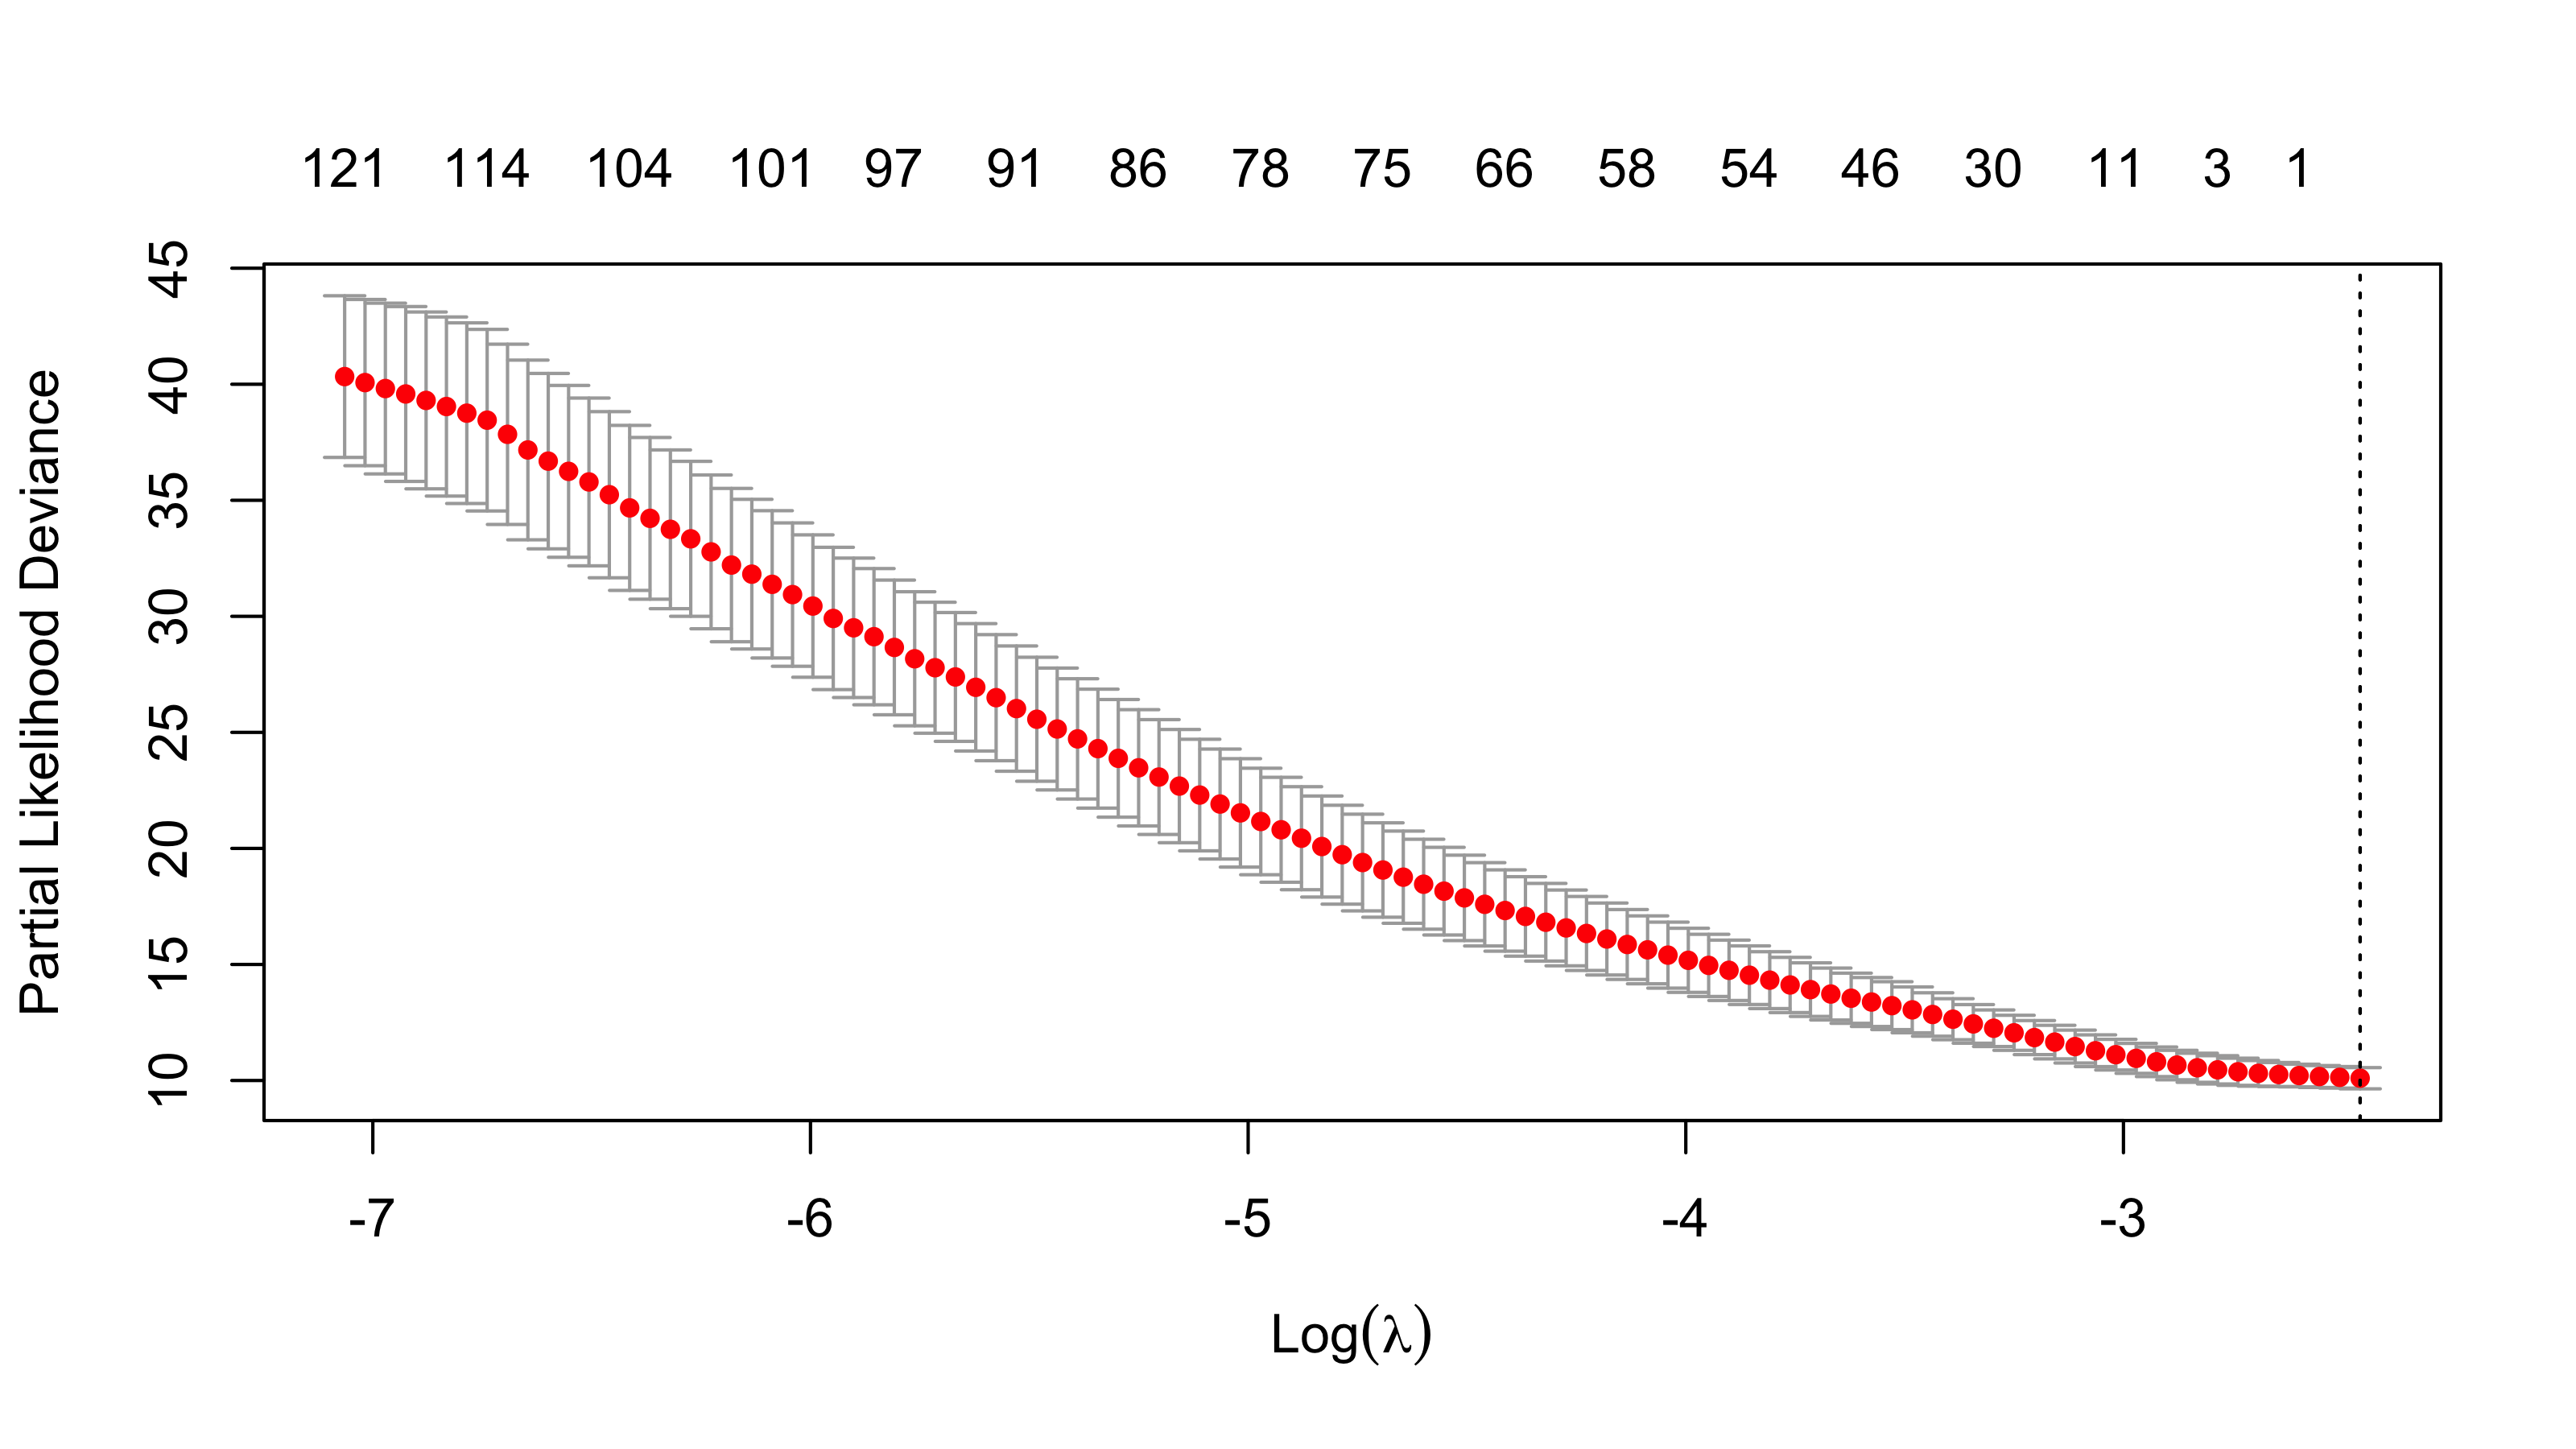
\includegraphics[keepaspectratio]{selection-1SE_files/figure-pdf/unnamed-chunk-4-1.png}}
\end{center}

\begin{Shaded}
\begin{Highlighting}[]
\CommentTok{\# Print selection}
\NormalTok{cc\_lasso\_min\_nc }\OtherTok{\textless{}{-}} \FunctionTok{coef}\NormalTok{(cox\_lasso\_nc, }\AttributeTok{s =}\NormalTok{ cox\_lasso\_nc}\SpecialCharTok{$}\NormalTok{lambda.min)}

\NormalTok{select\_vars\_lasso\_nc }\OtherTok{\textless{}{-}}\NormalTok{ cc\_lasso\_min\_nc}\SpecialCharTok{@}\NormalTok{Dimnames[[}\DecValTok{1}\NormalTok{]][}\SpecialCharTok{{-}}\DecValTok{1}\NormalTok{][cc\_lasso\_min\_nc}\SpecialCharTok{@}\NormalTok{i]}

\NormalTok{selected\_coefs\_lasso\_nc }\OtherTok{\textless{}{-}}\NormalTok{ cc\_lasso\_min\_nc}\SpecialCharTok{@}\NormalTok{x}

\FunctionTok{names}\NormalTok{(selected\_coefs\_lasso\_nc) }\OtherTok{\textless{}{-}}\NormalTok{ select\_vars\_lasso\_nc}

\NormalTok{selected\_coefs\_lasso\_nc}
\end{Highlighting}
\end{Shaded}

\begin{verbatim}
#> named numeric(0)
\end{verbatim}

\begin{Shaded}
\begin{Highlighting}[]
\CommentTok{\# Model w 1SE below}

\NormalTok{cox\_lambda\_min\_nc }\OtherTok{\textless{}{-}}\NormalTok{ cox\_lasso\_nc}\SpecialCharTok{$}\NormalTok{lambda.min}
\NormalTok{cox\_lambda\_min\_nc\_idx }\OtherTok{\textless{}{-}} \FunctionTok{which}\NormalTok{(cox\_lambda\_min\_nc }\SpecialCharTok{==}\NormalTok{ cox\_lasso\_nc}\SpecialCharTok{$}\NormalTok{lambda)}
\NormalTok{dev\_cox\_lambda\_nc }\OtherTok{\textless{}{-}}\NormalTok{ cox\_lasso\_nc}\SpecialCharTok{$}\NormalTok{cvm[cox\_lambda\_min\_nc\_idx]}
\NormalTok{se\_cox\_lambda\_nc }\OtherTok{\textless{}{-}}\NormalTok{ cox\_lasso\_nc}\SpecialCharTok{$}\NormalTok{cvsd[cox\_lambda\_min\_nc\_idx]}
\NormalTok{cox\_lambda\_min\_minus\_se\_idx }\OtherTok{\textless{}{-}} \FunctionTok{which.min}\NormalTok{(}\FunctionTok{abs}\NormalTok{(cox\_lasso\_nc}\SpecialCharTok{$}\NormalTok{cvm }\SpecialCharTok{{-}}\NormalTok{ (dev\_cox\_lambda\_nc }\SpecialCharTok{+}\NormalTok{ se\_cox\_lambda\_nc)))}
\NormalTok{cox\_lambda\_min\_minus\_se }\OtherTok{\textless{}{-}}\NormalTok{ cox\_lasso\_nc}\SpecialCharTok{$}\NormalTok{lambda[cox\_lambda\_min\_minus\_se\_idx]}

\NormalTok{cc\_lasso\_min\_minus\_se\_nc }\OtherTok{\textless{}{-}} \FunctionTok{coef}\NormalTok{(cox\_lasso\_nc, }\AttributeTok{s =}\NormalTok{ cox\_lambda\_min\_minus\_se)}

\NormalTok{select\_vars\_lasso\_nc }\OtherTok{\textless{}{-}}\NormalTok{ cc\_lasso\_min\_minus\_se\_nc}\SpecialCharTok{@}\NormalTok{Dimnames[[}\DecValTok{1}\NormalTok{]][}\SpecialCharTok{{-}}\DecValTok{1}\NormalTok{][cc\_lasso\_min\_minus\_se\_nc}\SpecialCharTok{@}\NormalTok{i]}

\NormalTok{selected\_coefs\_lasso\_nc }\OtherTok{\textless{}{-}}\NormalTok{ cc\_lasso\_min\_minus\_se\_nc}\SpecialCharTok{@}\NormalTok{x}

\FunctionTok{names}\NormalTok{(selected\_coefs\_lasso\_nc) }\OtherTok{\textless{}{-}}\NormalTok{ select\_vars\_lasso\_nc}

\CommentTok{\# Print corresponding variables}

\NormalTok{selected\_coefs\_lasso\_nc}
\end{Highlighting}
\end{Shaded}

\begin{verbatim}
#>       seq121       seq560       seq580       seq634 
#> -0.071100573 -0.001752633  0.082900786  0.646168945
\end{verbatim}




\end{document}
